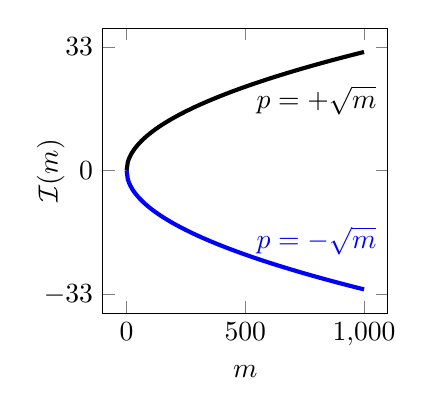
\begin{tikzpicture}
\begin{axis}
[scatter/classes={ a={mark=o,draw=blue}}, xlabel=$m$, ylabel=$\mathcal{I}(m)$,
y label style={at={(axis description cs:-0.1,0.5)},anchor=south},
  height=5.2cm,
  width=5.2cm,
  ytick={-33,0,33}]
\addplot[samples=200, line width=1.5pt, domain = 0:1000, color=black] plot(\x,{sqrt(\x)}) node[pos=0.8,inner sep=7pt, below] {$ p=+\sqrt{m} $};
\addplot[samples=200, line width=1.5pt, domain = 0:1000, color=blue] plot(\x,{-sqrt(\x)}) node[pos=0.8,inner sep=7pt, above] {$ p=-\sqrt{m} $};
\end{axis}
	%\draw[->] (-3,0)--(3,0) node[right]{$y$};
	%\draw[->] (0,-2)--(0,4) node[left]{$x$};
	%\draw[smooth, line width=1.5pt, domain = 0:3, color=blue] plot(\x,{sqrt(\x)}) node[right] {$ x=\sqrt{(x)} $};
	%\draw[smooth, line width=1.5pt, domain = 0:3, color=red] plot(\x,{-sqrt(\x)}) node[right] {$ y=-\sqrt{x} $};
\end{tikzpicture}
